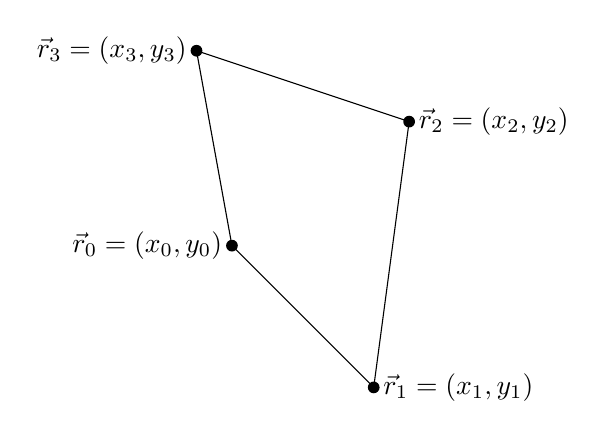
\begin{tikzpicture}[scale=2.25]
  \coordinate (zero) at (0, 0);
  \coordinate (one) at (0.8, -0.8);
  \coordinate (two) at (1, 0.7);
  \coordinate (three) at (-0.2, 1.1);
  \draw
    (zero) node[left] {$\vec{r}_0 = (x_0, y_0)$}
    -- (one) node[right] {$\vec{r}_1 = (x_1, y_1)$}
    -- (two) node[right] {$\vec{r}_2 = (x_2, y_2)$}
    -- (three) node[left] {$\vec{r}_3 = (x_3, y_3)$}
    -- cycle;
  \foreach \n in {zero,one,two,three}
    \node at (\n)[circle,fill,inner sep=1.5pt]{};
\end{tikzpicture}
